\documentclass[10pt]{article}
\usepackage[a4paper,margin=1.7cm]{geometry}
\usepackage{amsmath,amssymb,amsthm,mathtools}
\usepackage{booktabs,tabularx,array,multirow}
\usepackage{microtype}
\usepackage{graphicx}
\usepackage{tikz}
\usetikzlibrary{arrows.meta,positioning,fit,calc}
\usepackage{pgfplots}
\pgfplotsset{compat=1.18}
\usepackage{xcolor}
\usepackage{hyperref}
\usepackage{cleveref}
\usepackage{enumitem}
\usepackage{siunitx}
\newtheorem{theorem}{Theorem}
\newtheorem{proposition}{Proposition}
\newtheorem{lemma}{Lemma}
\newcommand{\KL}{D_{\mathrm{KL}}}
\newcommand{\RR}{\mathcal{R}}
\newcommand{\CC}{\mathcal{C}}
\newcommand{\FR}{\mathrm{FR}}
\newcommand{\E}{\mathbb{E}}
\title{Information-Geometric Robustness for Cachin-Secure Steganography}
\author{St\'ephane G. R. Ekodeck}
\date{}

\begin{document}
\maketitle

\begin{abstract}
Information-theoretic steganography characterizes passive-warden security through the divergence between cover and stego distributions, while practical image sources vary with acquisition and processing conditions. This work develops a source--embedding information-geometric framework that preserves Cachin's exact relative-entropy criterion while exposing the sensitivity of a fixed embedding design to cover-source displacement. The method defines an exact Cachin security field, equips the source manifold with Fisher--Rao geometry, derives a finite-radius robust risk, and optimizes an eight-stratum ternary embedding under that risk. The formal analysis recovers the established embedding-direction Fisher regime locally and proves that a source-sensitive design on a positive nominal Cachin boundary loses same-budget robust feasibility for sufficiently small source perturbations. Controlled and BOSSBase experiments separate nominal security from source robustness: an independent iso-Cachin confirmation yields median central dispersion \(D_{80}=0.1902\) at the stress radius, while empirical-PMF source geometry on BOSSBase yields \(D_{80}=0.4817\) and \(0.5308\). At the same certified robust risk, information-geometric reallocation increases the ideal rate envelope by \(2.8849\%\) and \(16.5025\%\); at the same ideal payload, it reduces certified worst-case risk by \(6.7272\%\) and \(38.1360\%\). A complete 20,000-condition STC campaign achieves 100\% coding success at the lower budget and at least 99.96\% at the higher budget, with zero bit error on every successfully decoded codeword. These results show that exact nominal Cachin security can conceal substantial source-robustness heterogeneity and that the revealed geometry can be used to construct non-scalar robust embedding allocations.
\end{abstract}

\noindent\textbf{Keywords:} steganography; Cachin security; information geometry; Fisher--Rao metric; cover-source mismatch; robust optimization; syndrome-trellis codes.

\section{Introduction}
Cachin's information-theoretic model formulates passive steganographic detection as hypothesis testing and measures security by relative entropy between the cover and stego distributions \cite{cachin2004}. For a cover law \(P_C\) and an induced stego law \(P_S\), the canonical orientation used throughout this paper is
\begin{equation}
  \KL(P_C\Vert P_S).
  \label{eq:cachin}
\end{equation}
The criterion is exact for a specified source--design pair, yet operational image sources vary because acquisition devices and processing pipelines vary. The cover-source mismatch literature shows that such source changes materially affect steganalysis and can reverse conclusions obtained on a single source \cite{kodovsky2011,giboulot2020,mallet2024}.

Local Fisher information already has a precise role in steganography. Filler and Fridrich characterized mutually independent embedding and linked the local quadratic behavior of KL divergence to Fisher information with respect to embedding rate \cite{filler2009icas,filler2009ih}. Ker estimated related local quantities on real images \cite{ker2009}, and MiPOD later used a local statistical detectability model to derive content-adaptive allocations \cite{sedighi2016}. These results motivate a different question: what structure appears when the embedding design is held fixed and the \emph{cover source} moves?

We answer this question by defining an exact source--embedding security field and equipping its source argument with Fisher--Rao geometry. The construction retains \cref{eq:cachin} as the governing security quantity, but augments it with source-direction sensitivity and a finite-radius worst-case risk. \Cref{fig:framework} summarizes the resulting separation between exact nominal security, embedding-direction local Fisher behavior, and source-direction robust design.

\begin{figure}[t]
\centering
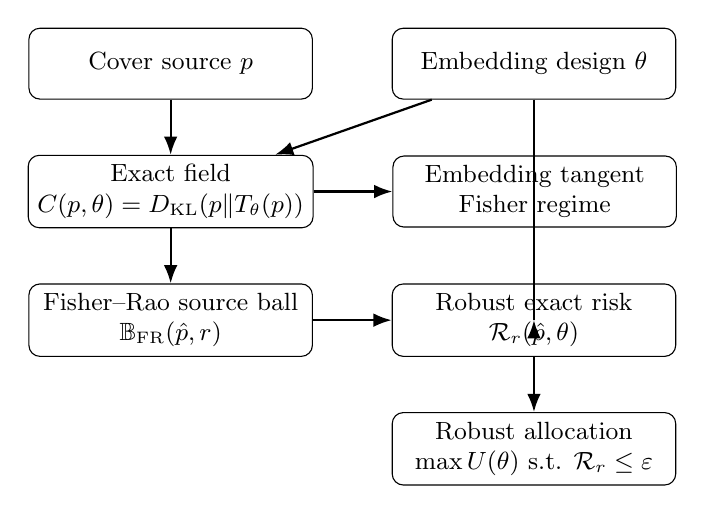
\begin{tikzpicture}[node distance=7mm and 10mm,>=Latex,
 box/.style={draw,rounded corners,align=center,minimum width=3.6cm,minimum height=9mm,font=\small},
 arr/.style={->,thick}]
\node[box] (source) {Cover source \(p\)};
\node[box,right=of source] (embed) {Embedding design \(\theta\)};
\node[box,below=of source] (field) {Exact field\\\(C(p,\theta)=\KL(p\Vert T_\theta(p))\)};
\node[box,right=of field] (fisher) {Embedding tangent\\Fisher regime};
\node[box,below=of field] (ball) {Fisher--Rao source ball\\\(\mathbb B_{\FR}(\hat p,r)\)};
\node[box,right=of ball] (risk) {Robust exact risk\\\(\RR_r(\hat p,\theta)\)};
\node[box,below=of risk] (opt) {Robust allocation\\\(\max U(\theta)\) s.t. \(\RR_r\le\varepsilon\)};
\draw[arr] (source) -- (field);
\draw[arr] (embed) -- (field);
\draw[arr] (field) -- (fisher);
\draw[arr] (field) -- (ball);
\draw[arr] (ball) -- (risk);
\draw[arr] (embed) |- (risk);
\draw[arr] (risk) -- (opt);
\end{tikzpicture}
\caption{Source--embedding security construction. Exact Cachin risk remains the central scalar security quantity; Fisher--Rao geometry is applied to source displacement and then used as a robust design constraint.}
\label{fig:framework}
\end{figure}

The contribution is threefold. First, we formalize source-direction Fisher--Rao sensitivity of exact Cachin risk and establish a boundary-separation theorem that directly constrains robust embedding design. Second, we instantiate the framework in a quantized residual-PMF model with eight content strata and certify worst-case risks by independent high-resolution searches. Third, we connect the model to operational coding through real STC encoding and exact message recovery. The evidence sequence is shown in \cref{fig:evidence}; it was designed to retain both favorable and boundary findings rather than selecting only regimes with large gains.

\begin{figure}[t]
\centering
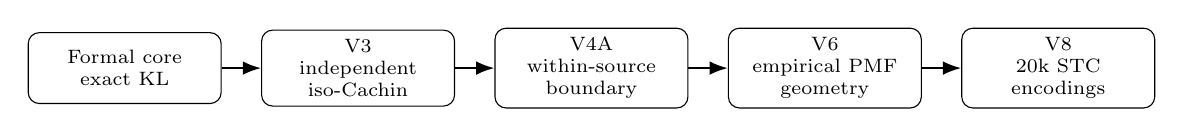
\begin{tikzpicture}[>=Latex,node distance=5mm,
 s/.style={draw,rounded corners,align=center,minimum width=2.45cm,minimum height=9mm,font=\scriptsize}]
\node[s] (v1) {Formal core\\exact KL};
\node[s,right=of v1] (v3) {V3\\independent\\iso-Cachin};
\node[s,right=of v3] (v4) {V4A\\within-source\\boundary};
\node[s,right=of v4] (v6) {V6\\empirical PMF\\geometry};
\node[s,right=of v6] (v8) {V8\\20k STC\\encodings};
\draw[->,thick] (v1)--(v3);
\draw[->,thick] (v3)--(v4);
\draw[->,thick] (v4)--(v6);
\draw[->,thick] (v6)--(v8);
\end{tikzpicture}
\caption{Evidence sequence used in the study. V4A is retained as a boundary result: within-source variability was measurable but below the frozen materiality threshold, motivating the fuller empirical-PMF source model used in V6.}
\label{fig:evidence}
\end{figure}

\section{Positioning}
\Cref{tab:positioning} separates the present construction from the closest established lines. Cachin supplies the exact security scalar \cite{cachin2004}; Filler--Fridrich and Ker characterize local embedding-direction Fisher behavior \cite{filler2009icas,filler2009ih,ker2009}; MiPOD derives a practical local allocation under a Gaussian cover model \cite{sedighi2016}. Cover-model incompleteness and source mismatch are well documented \cite{kodovsky2011,sedighi2016boss,giboulot2020,mallet2024}. A robust-optimization formalization has also been proposed on the steganalyst side \cite{sepak2022}. Fisher--Rao variational classes have independently been used for robustness analysis in uncertainty quantification \cite{ketema2025}. The present object is the sender-side combination of exact Cachin risk, source-manifold geometry, and a finite-radius robust embedding constraint.

\begin{table}[t]
\centering
\caption{Positioning relative to established components.}
\label{tab:positioning}
\small
\begin{tabularx}{\linewidth}{@{}lXXX@{}}
\toprule
Work & Primary object & Direction of variation & Design consequence\\
\midrule
Cachin \cite{cachin2004} & Exact \(\KL(P_C\Vert P_S)\) & Fixed source/design pair & \(\varepsilon\)-security\\
Filler--Fridrich \cite{filler2009icas,filler2009ih} & Steganographic Fisher information & Embedding-rate tangent & Local security/capacity analysis\\
MiPOD \cite{sedighi2016} & Statistical detectability model & Per-pixel change rates & Content-adaptive allocation\\
CSM literature \cite{giboulot2020,sepak2022,mallet2024} & Source mismatch / detector transfer & Training--test source shift & Detector-side robustness/adaptation\\
This work & Exact source--embedding risk field & Cover-source Fisher--Rao displacement & Sender-side robust allocation\\
\bottomrule
\end{tabularx}
\end{table}

\section{Formal model}
Let \(\mathcal P=\Delta_{K-1}^{\circ}\) be the interior categorical source manifold with Fisher metric
\begin{equation}
 g_p(u,v)=\sum_{i=1}^{K}\frac{u_i v_i}{p_i},
 \qquad \sum_i u_i=\sum_i v_i=0.
 \label{eq:fishermetric}
\end{equation}
Let \(\Theta\) parameterize an embedding family and \(T_\theta(p)\) denote the induced stego law. Define the source--embedding security field
\begin{equation}
  C(p,\theta)=\KL\!\left(p\Vert T_\theta(p)\right).
  \label{eq:field}
\end{equation}
For a nominal source \(\hat p\), let
\begin{equation}
 \mathbb B_{\FR}(\hat p,r)=
 \{p:d_{\FR}(p,\hat p)\le r\},
 \quad
 d_{\FR}(p,q)=2\arccos\sum_i\sqrt{p_iq_i},
 \label{eq:frball}
\end{equation}
and define the robust exact-Cachin risk
\begin{equation}
 \RR_r(\hat p,\theta)
 =
 \sup_{p\in\mathbb B_{\FR}(\hat p,r)}
 \KL\!\left(p\Vert T_\theta(p)\right).
 \label{eq:robustrisk}
\end{equation}
The zero-radius identity \(\RR_0(\hat p,\theta)=C(\hat p,\theta)\), monotonicity in \(r\), and the uniform implication \(\RR_r\le\varepsilon\Rightarrow C(p,\theta)\le\varepsilon\) for every \(p\) in the declared ball follow directly from \cref{eq:robustrisk}. We retain these statements as propositions because their role is compatibility and semantics.

For a smooth embedding curve \(\theta(\beta)\) satisfying \(T_{\theta(0)}(p)=p\), standard regularity gives
\begin{equation}
 C(p,\theta(\beta))
 =
 \frac{\beta^2}{2}I_{\rm emb}(p;\dot\theta(0))+O(\beta^3),
 \label{eq:fillerrecovery}
\end{equation}
which recovers the established embedding-direction Fisher regime under the assumptions used by Filler and Fridrich \cite{filler2009icas,filler2009ih}. The source-direction quantity is different:
\begin{equation}
 S_{\rm src}(p,\theta)
 =
 \left\|\operatorname{grad}^{\FR}_{p}C(p,\theta)\right\|_{g_p}.
 \label{eq:ssrc}
\end{equation}

For a row-stochastic categorical channel \(B\), \(q=pB\), set
\begin{equation}
 a_k=
 \log\frac{p_k}{q_k}+1-\sum_j B_{kj}\frac{p_j}{q_j}.
 \label{eq:ak}
\end{equation}
Direct differentiation and projection onto the simplex tangent space yield
\begin{equation}
 (\operatorname{grad}^{\FR}C_B)_k
 =p_k[a_k-C_B(p)],
 \qquad
 S_{\rm src}^2
 =\sum_k p_k[a_k-C_B(p)]^2.
 \label{eq:frgradient}
\end{equation}
For a replacement channel with fixed output \(q\), \cref{eq:frgradient} reduces to the relative-entropy variance \(V(p\Vert q)\).

\begin{theorem}[Source-mismatch separation on a nominal Cachin boundary]
\label{thm:separation}
Let \(\hat p\) be an interior point of a finite categorical source manifold equipped with the Fisher metric. Assume \(T_\theta\) is \(C^2\) in a neighborhood of \(\hat p\), the induced stego law has positive support there, and
\[
C(\hat p,\theta)=\varepsilon>0,
\qquad
S_{\rm src}(\hat p,\theta)>0.
\]
Then there exists \(r_0>0\) such that, for every \(0<r<r_0\),
\[
\RR_r(\hat p,\theta)>\varepsilon.
\]
\end{theorem}

\begin{proof}
Let \(v\) be the unit Fisher--Rao tangent vector aligned with
\(\operatorname{grad}^{\FR}_{p}C(\hat p,\theta)\), and let \(\gamma(t)\) be the Fisher--Rao geodesic with \(\gamma(0)=\hat p\) and \(\dot\gamma(0)=v\). Interiority and positive induced support provide a normal neighborhood in which \(C(\cdot,\theta)\) is \(C^2\). Taylor expansion along \(\gamma\) gives
\[
C(\gamma(t),\theta)
=
\varepsilon+t\,S_{\rm src}(\hat p,\theta)+O(t^2).
\]
Because \(S_{\rm src}>0\), the right-hand side exceeds \(\varepsilon\) for every sufficiently small positive \(t\). For such \(t\), \(d_{\FR}(\gamma(t),\hat p)=t\); hence \(\gamma(t)\in\mathbb B_{\FR}(\hat p,t)\), and the supremum defining \(\RR_t\) is strictly larger than \(\varepsilon\).
\end{proof}

\Cref{thm:separation} constrains the design space: a source-sensitive solution that merely saturates a positive nominal budget cannot retain that same budget under every sufficiently small source displacement. Robust design therefore introduces nominal slack or moves toward source-stationary directions. This is the exact mechanism used by the optimization below.

\section{Quantized image witness}
The image witness uses a non-overlapping \(3\times3\) carrier lattice. Only center pixels are modifiable; the four-neighbor rounded predictor remains unchanged by a center modification. Let the integer residual be
\[
R=X_c-\operatorname{round}\!\left(\frac{N+S+E+W}{4}\right).
\]
Eight frozen context strata are formed from the dispersion of the eight surrounding pixels. Within stratum \(g\), a symmetric ternary embedding uses
\[
\Pr(\Delta=+1)=\beta_g,\quad
\Pr(\Delta=-1)=\beta_g,\quad
\Pr(\Delta=0)=1-2\beta_g.
\]
For an empirical residual PMF \(p_g(k)\), the induced stego PMF is exact:
\begin{equation}
q_{g,\beta}(k)
=(1-2\beta_g)p_g(k)
+\beta_gp_g(k-1)
+\beta_gp_g(k+1).
\label{eq:pmfchannel}
\end{equation}
The ideal ternary payload envelope is
\begin{equation}
R_{\rm ideal}(\boldsymbol\beta)
=
\sum_g w_g H_3(\beta_g),
\quad
H_3(\beta)=-2\beta\log_2\beta-(1-2\beta)\log_2(1-2\beta).
\label{eq:idealrate}
\end{equation}
The operational stage later replaces this entropy envelope by actual STC message bits.

The final V6 source geometry is learned from empirical residual-PMF shape variation across camera sources. Three Fisher modes explain \(97.85\%\) of the measured inter-camera Fisher energy, and calibration gives \(r_{\rm shape}=0.237503\). The robust design solves
\begin{equation}
\max_{\boldsymbol\beta}R_{\rm ideal}(\boldsymbol\beta)
\quad\text{s.t.}\quad
\sup_{\delta\in\mathcal U(r_{\rm shape})}
C(\delta,\boldsymbol\beta)\le\varepsilon,
\label{eq:robustopt}
\end{equation}
with independent Sobol-sphere certification at 131,072 directions.

\section{Experimental protocol}
BOSSBase 1.01 was reconstructed and CRC-validated as 10,000 grayscale \(512\times512\) PGM images. A filename-hash split fixes 3,500 fit images, 1,500 calibration images, and 5,000 holdout images before model estimation. Stratum boundaries, empirical PMFs, source modes, radii, design seeds, two Cachin budgets \(\varepsilon\in\{2\times10^{-4},8\times10^{-4}\}\), and numerical decision rules were frozen before the corresponding confirmatory stages.

The causal comparator is \emph{uniform safety shrinkage}: starting from the nominal exact-Cachin optimum, all \(\beta_g\) are multiplied by the largest common scalar that satisfies the same robust budget. This comparator tests whether the geometric optimizer learns a genuinely different allocation rather than merely reducing the payload.

A separate independent iso-Cachin study generates 128 positive eight-dimensional allocations per profile/budget and projects each onto the same exact nominal Cachin boundary. Robust inflation \(J=\RR_r/\varepsilon\) is summarized by
\[
D_{80}=Q_{90}(J)-Q_{10}(J).
\]
The image-domain operational screen uses paired payloads. The final coding experiment uses actual STC messages at \(90\%\) of the frozen ideal payload and retains coding failures in the denominator.

\section{Results}
\subsection{Controlled and confirmatory behavior}
Across 48 frozen controlled-grid cells, the robust optimizer satisfies the robust budget in every cell and differs from a scalar rescaling of the nominal allocation for every positive-radius condition. The median rate gain over uniform shrinkage is \(0.436\%\), while the strongest heterogeneous finite-radius conditions approach \(4\%\). \Cref{fig:grid-gain} and \cref{tab:grid-summary} make the regime dependence explicit.

\begin{figure}[t]
\centering
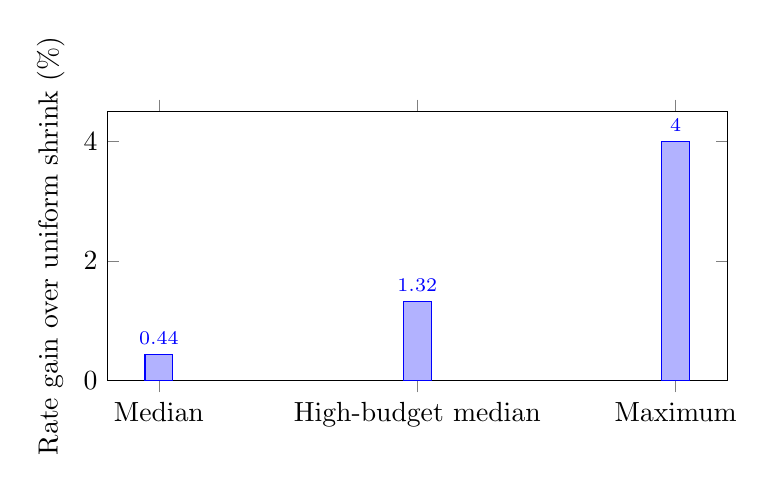
\begin{tikzpicture}
\begin{axis}[
ybar, width=.78\linewidth,height=5cm,
ylabel={Rate gain over uniform shrink (\%)},
symbolic x coords={Median,High-budget median,Maximum},
xtick=data,ymin=0,ymax=4.5,
nodes near coords,
every node near coord/.append style={font=\scriptsize},
]
\addplot coordinates {(Median,0.436) (High-budget median,1.32) (Maximum,4.00)};
\end{axis}
\end{tikzpicture}
\caption{Controlled-grid rate advantage over uniform safety shrinkage. The effect is small near the local/low-radius regime and becomes larger for heterogeneous finite-displacement regimes.}
\label{fig:grid-gain}
\end{figure}

\begin{table}[t]
\centering
\caption{Controlled and independent confirmatory evidence.}
\label{tab:grid-summary}
\small
\begin{tabular}{@{}lrr@{}}
\toprule
Quantity & Result & Interpretation\\
\midrule
Frozen controlled cells & 48 & full grid retained\\
Positive-radius budget violations & 0 & feasibility maintained\\
Median rate gain & 0.436\% & modest central effect\\
Cells with gain \(>2\%\) & 11.1\% & effect concentrated by regime\\
Independent V3 median \(D_{80}\) at \(r=0.12\) & 0.1902 & iso-Cachin heterogeneity confirmed\\
\bottomrule
\end{tabular}
\end{table}

The independent V3 sample confirms the structural prediction: allocations with the same exact nominal \(\varepsilon\) can have materially different source-robust risks. This is the empirical counterpart of \cref{thm:separation}; the theorem predicts loss of same-budget robustness under nonzero source sensitivity, while the experiment quantifies how strongly different boundary allocations separate.

\subsection{Natural-source geometry and boundary findings}
The first BOSSBase calibration (V4A) used within-source block variation and produced \(r^\star=0.03795\). Its \(D_{80}\) values, \(0.0218\) and \(0.0387\), remained below the frozen materiality threshold \(0.05\). This boundary finding establishes that ordinary within-source sampling variation is too small to support a large-effect narrative.

A camera-aware source model exposed much larger inter-source displacement, but direct empirical PMF evaluation showed that a log-scale-only nuisance family missed residual-shape variation at the lower budget. V6 therefore represents source shifts directly in empirical residual-PMF Fisher coordinates. With three modes explaining \(97.85\%\) of inter-camera Fisher energy, V6 yields \(D_{80}=0.4817\) and \(0.5308\), as shown in \cref{fig:natural-d80} and summarized in \cref{tab:natural-results}.

\begin{figure}[t]
\centering
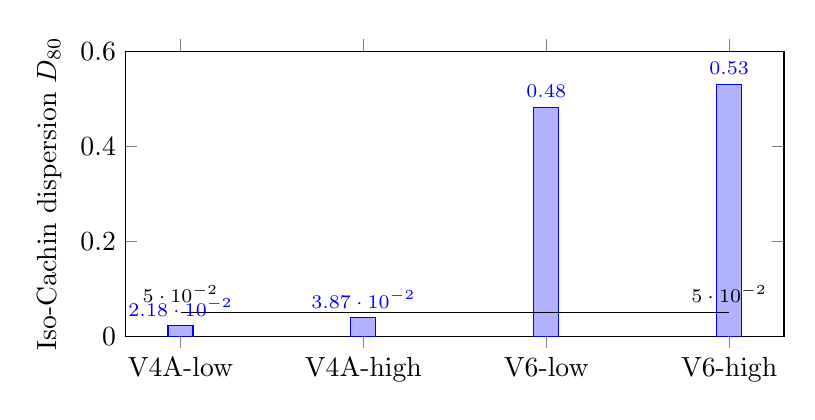
\begin{tikzpicture}
\begin{axis}[
ybar,bar width=9pt,width=.82\linewidth,height=5.2cm,
ylabel={Iso-Cachin dispersion \(D_{80}\)},
symbolic x coords={V4A-low,V4A-high,V6-low,V6-high},
xtick=data,ymin=0,ymax=.60,
nodes near coords,
every node near coord/.append style={font=\scriptsize},
]
\addplot coordinates {(V4A-low,0.0218) (V4A-high,0.0387) (V6-low,0.4817) (V6-high,0.5308)};
\addplot[domain=-1:4,samples=2,sharp plot] coordinates {(V4A-low,0.05) (V6-high,0.05)};
\end{axis}
\end{tikzpicture}
\caption{Natural-source iso-Cachin dispersion. V4A measures within-source variability; V6 models empirical PMF shape variation across acquisition sources. The horizontal reference is the predeclared \(D_{80}=0.05\) materiality threshold.}
\label{fig:natural-d80}
\end{figure}

\begin{table}[t]
\centering
\caption{Natural-source robust-design results after independent 131,072-direction certification.}
\label{tab:natural-results}
\small
\begin{tabular}{@{}lrr@{}}
\toprule
Quantity & \(\varepsilon=2\times10^{-4}\) & \(\varepsilon=8\times10^{-4}\)\\
\midrule
V6 \(D_{80}\) & 0.481655 & 0.530772\\
Uniform-shrink rate & 0.532112 & 0.720079\\
Robust rate & 0.547463 & 0.838909\\
Rate gain at same robust risk & 2.8849\% & 16.5025\%\\
Worst-risk reduction at same ideal payload & 6.7272\% & 38.1360\%\\
Non-scalar allocation residual & 0.159757 & 0.143791\\
\bottomrule
\end{tabular}
\end{table}

The two dual views of the design consequence are plotted in \cref{fig:dual-benefit}. The large-budget regime shows a substantial geometric advantage, whereas the lower budget retains a smaller but positive benefit. This pattern is consistent with the controlled grid: the framework is most useful when finite source displacement and source heterogeneity create exploitable directions along the nominal security frontier.

\begin{figure}[t]
\centering
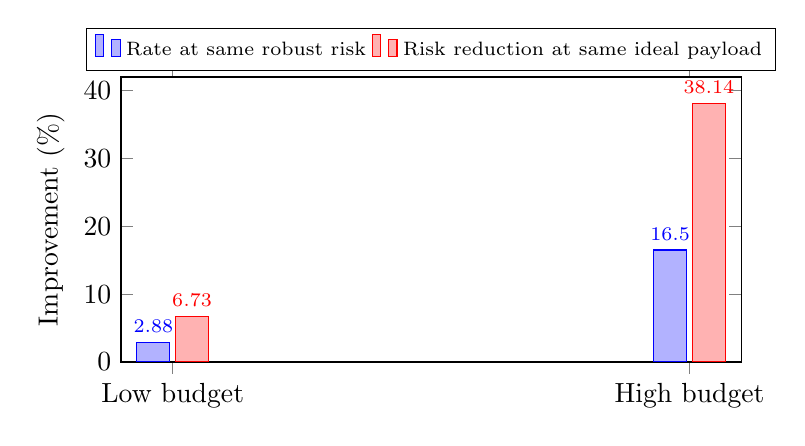
\begin{tikzpicture}
\begin{axis}[
ybar,bar width=12pt,width=.78\linewidth,height=5.2cm,
ylabel={Improvement (\%)},
symbolic x coords={Low budget,High budget},
xtick=data,ymin=0,ymax=42,
legend style={at={(0.5,1.02)},anchor=south,legend columns=2,font=\scriptsize},
nodes near coords,
every node near coord/.append style={font=\scriptsize},
]
\addplot coordinates {(Low budget,2.8849) (High budget,16.5025)};
\addplot coordinates {(Low budget,6.7272) (High budget,38.1360)};
\legend{Rate at same robust risk,Risk reduction at same ideal payload}
\end{axis}
\end{tikzpicture}
\caption{Dual operational meaning of the same geometry: additional rate under a fixed robust security budget, or additional security margin at a fixed ideal payload.}
\label{fig:dual-benefit}
\end{figure}

\subsection{Image realization and actual message coding}
The V7 development screen realizes the paired allocations stochastically on 800 frozen BOSSBase development/calibration images. The lightweight residual detector remains close to chance for both allocations at matched ideal payload, as reported in \cref{tab:operational}. These results verify image realization and provide a low-cost detector sanity check; detector-facing conclusions are reserved for the strong steganalysis layer discussed later.

\begin{table}[t]
\centering
\caption{V7 matched-ideal-payload image screening.}
\label{tab:operational}
\small
\begin{tabular}{@{}lrrrr@{}}
\toprule
Budget & Method & Ideal bpp & Change/eligible & AUC\\
\midrule
\(2\times10^{-4}\) & Uniform shrink & 0.058046 & 0.107950 & 0.505022\\
\(2\times10^{-4}\) & IG matched & 0.058046 & 0.114292 & 0.502361\\
\(8\times10^{-4}\) & Uniform shrink & 0.078550 & 0.157984 & 0.508172\\
\(8\times10^{-4}\) & IG matched & 0.078550 & 0.168414 & 0.502589\\
\bottomrule
\end{tabular}
\end{table}

The final V8 experiment replaces entropy-only payload with actual STC messages over 5,000 images and four budget/method conditions, for 20,000 encodings. \Cref{tab:stc} retains every coding failure. At the lower budget both allocations decode all 5,000 messages. At the higher budget uniform shrink has two failures and the information-geometric allocation has one. Every codeword classified as successfully decoded has BER zero. The all-bit BER values in \cref{tab:stc} count errors in the retained failed codewords.

\begin{table}[t]
\centering
\caption{Complete V8 STC coding results; failures remain in the denominator.}
\label{tab:stc}
\small
\begin{tabular}{@{}llrrrr@{}}
\toprule
Budget & Method & Success & All-bit BER & Message bpp & Change frac.\\
\midrule
\(2\times10^{-4}\) & Uniform shrink & 5000/5000 & 0 & 0.052170 & 0.101895\\
\(2\times10^{-4}\) & IG matched & 5000/5000 & 0 & 0.052170 & 0.106036\\
\(8\times10^{-4}\) & Uniform shrink & 4998/5000 & \(8.81\times10^{-5}\) & 0.070600 & 0.146545\\
\(8\times10^{-4}\) & IG matched & 4999/5000 & \(5.11\times10^{-5}\) & 0.070600 & 0.153574\\
\bottomrule
\end{tabular}
\end{table}

At matched message payload, the information-geometric allocation uses slightly more modifications: the paired mean change-fraction increase is \(0.00414\) at the lower budget and \(0.00703\) at the higher budget. Mean PSNR decreases by \(0.171\) and \(0.200\) dB, respectively, while mean embedding distortion cost is lower for the information-geometric allocation in both conditions. These image-change diagnostics motivate a strong detector comparison at equal actual payload.

\section{Discussion}
The central result is a distinction between nominal security and source robustness. Cachin's \(\varepsilon\) remains the exact nominal security coordinate, but \cref{thm:separation} shows that a source-sensitive boundary design cannot retain the same budget throughout every sufficiently small Fisher--Rao neighborhood. The independent iso-Cachin experiments then show that this loss of margin is not uniform across designs: equal nominal KL can conceal materially different robustness.

The controlled grid and V4A are also informative. The median controlled rate gain is only \(0.436\%\), and within-source natural variability remains below the predeclared materiality threshold. The useful regime emerges when the uncertainty set represents genuine source heterogeneity rather than ordinary sampling fluctuation. The empirical-PMF V6 model captures residual-shape changes that the earlier scale-only model missed and yields both a strong iso-Cachin separation and an actionable non-scalar allocation.

The guarantee is tied to the declared empirical-PMF Fisher manifold and its calibrated radius. Cross-corpus transfer therefore serves as a test of how well that manifold covers a genuinely independent source, rather than as a re-fitting opportunity. The frozen BOWS2 protocol uses BOWS2 stratum masses and PMFs directly while retaining every BOSSBase-fitted geometric object. A source outside the declared manifold is interpreted as an external-transfer boundary of the fitted geometry.

Detector-facing validation forms a separate empirical layer. SRM with an ensemble classifier \cite{fridrich2012} and deep residual steganalysis such as SRNet \cite{boroumand2019} provide substantially stronger wardens than the V7 screen. Equal actual payload, source-disjoint evaluation, repeated seeds for deep models, confidence intervals, and retained coding failures are required for that layer. This separation keeps the information-theoretic guarantee, coding reliability, and empirical warden resistance as distinct measured properties.

\section{Limitations and external validity}
The finite-alphabet theorem applies to interior source distributions with smooth positive induced stego support. The image witness instantiates this model through eight residual strata and a finite empirical PMF support; finer contextual structure may reveal additional source directions. The calibrated Fisher subspace is learned from BOSSBase acquisition sources, so independent-source evaluation is necessary to measure its transfer range.

The current BOSSBase results establish the formal/design/coding chain and expose where within-source and scale-only models become insufficient. The final external-validity layer uses the frozen BOWS2 experiment, and the final detector-validity layer uses SRM+ensemble together with a repeated-seed deep detector. These two experiments determine how far the observed source-robust design benefit extends beyond the fitted BOSSBase geometry and under stronger empirical wardens.

\section{Conclusion}
This work embeds Cachin's exact relative-entropy security criterion in a source--embedding information-geometric framework. The resulting source-direction Fisher--Rao sensitivity yields a nontrivial design constraint: a source-sensitive solution on a positive nominal Cachin boundary loses same-budget robust feasibility under sufficiently small source displacement. Controlled and natural-image experiments confirm that nominally iso-Cachin designs can have substantially different robust risks, and empirical-PMF geometry turns that difference into certified non-scalar allocations. On BOSSBase, the robust allocation improves the ideal rate envelope by \(2.8849\%\) and \(16.5025\%\) at the two tested budgets, or reduces certified worst-case risk by \(6.7272\%\) and \(38.1360\%\) at matched ideal payload. A 20,000-condition STC experiment further shows reliable actual-message realization with the retained failures explicitly reported. The resulting framework provides a direct route from exact nominal steganographic security to source-aware robust embedding design.

\bibliographystyle{plain}
\bibliography{references}
\end{document}
